\documentclass[12pt]{article}
%%% DOCUMENT FORMATTING %%%
\usepackage[margin=1in]{geometry}
\usepackage{enumitem}
\setlength{\parindent}{0pt}
\newcommand{\disp}{\displaystyle}
\usepackage{multicol}

%%% HEADER %%%
\usepackage{fancyhdr}
\pagestyle{fancy}
\fancyhf{}
\lhead{MATH 1080}
\rhead{Vagnozzi}
\cfoot{\thepage}

%%% MATH NOTATION & SYMBOLS %%%
\usepackage{amssymb}
\usepackage{amsmath}
\newcommand{\R}{\mathbb{R}}
\newcommand{\N}{\mathbb{N}}
\newcommand{\Z}{\mathbb{Z}}
\newcommand{\lp}{\left(}
\newcommand{\rp}{\right)}
\newcommand{\ls}{\left[}
\newcommand{\rs}{\right]}
\newcommand{\lb}{\left\{}
\newcommand{\rb}{\right\}}
\newcommand{\arccot}{\text{arccot}}
\newcommand{\arccsc}{\text{arccsc}}
\newcommand{\arcsec}{\text{arcsec}}
\DeclareSymbolFont{matha}{OML}{txmi}{m}{it}% txfonts
\DeclareMathSymbol{\varv}{\mathord}{matha}{118} 

%%% TABLES %%%
\usepackage{colortbl}

%%% GRAPHS %%%
\usepackage{tikz}
\usepackage{pgfplots}
\pgfplotsset{compat=1.15}
\usepgfplotslibrary{fillbetween}
\usetikzlibrary{angles,quotes}

%%% ENVIRONMENTS %%%
\newcommand{\Example}{\paragraph{\Writinghand \hspace{0.1mm} Example.}}
\newcommand{\Examples}{\paragraph{\Writinghand \hspace{0.1mm} Examples.}}
\newcommand{\ExampleCont}{\paragraph{\Writinghand \hspace{0.1mm} Example (continued).}}
\newcommand{\ExamplesCont}{\paragraph{\Writinghand \hspace{0.1mm} Examples (continued).}}

\newcommand{\boxenv}[2]{
	\fbox{
	\begin{minipage}{0.97\textwidth}
	\vspace{2mm}	
	\paragraph{#1} #2
	\vspace{2mm}
	\end{minipage}
	}}

%%% FUN THINGS %%%
\newcommand*\tc[1]{\tikz[baseline=(char.base)]{
            \node[shape=circle,draw,inner sep=2pt] (char) {#1};}}
\usepackage{marvosym}

%%% MISC %%%
\usepackage{hyperref}


\setcounter{page}{169}

\begin{document}
\section*{12.2: Polar Coordinates}

\boxenv{Learning Objectives.}{Upon successful completion of Section 12.2, you will be able to\dots
		
	\begin{itemize}[leftmargin=6mm]
		\item Answer conceptual questions involving polar coordinates.
		\item Graph with polar coordinates and give alternate polar representations of polar points.
		\item Convert between polar and Cartesian coordinates.
		\item Convert between polar equations and Cartesian equations.
		\item Graph simple polar curves.
		\item Identify corresponding points given Cartesian and polar graphs of the same curve.
	\end{itemize}
	\vspace{-4mm}
}

\vspace{5mm}

\subsection*{Introduction to Polar Coordinates}

\newpage

\Example Plot the following polar coordinates.

\begin{center}
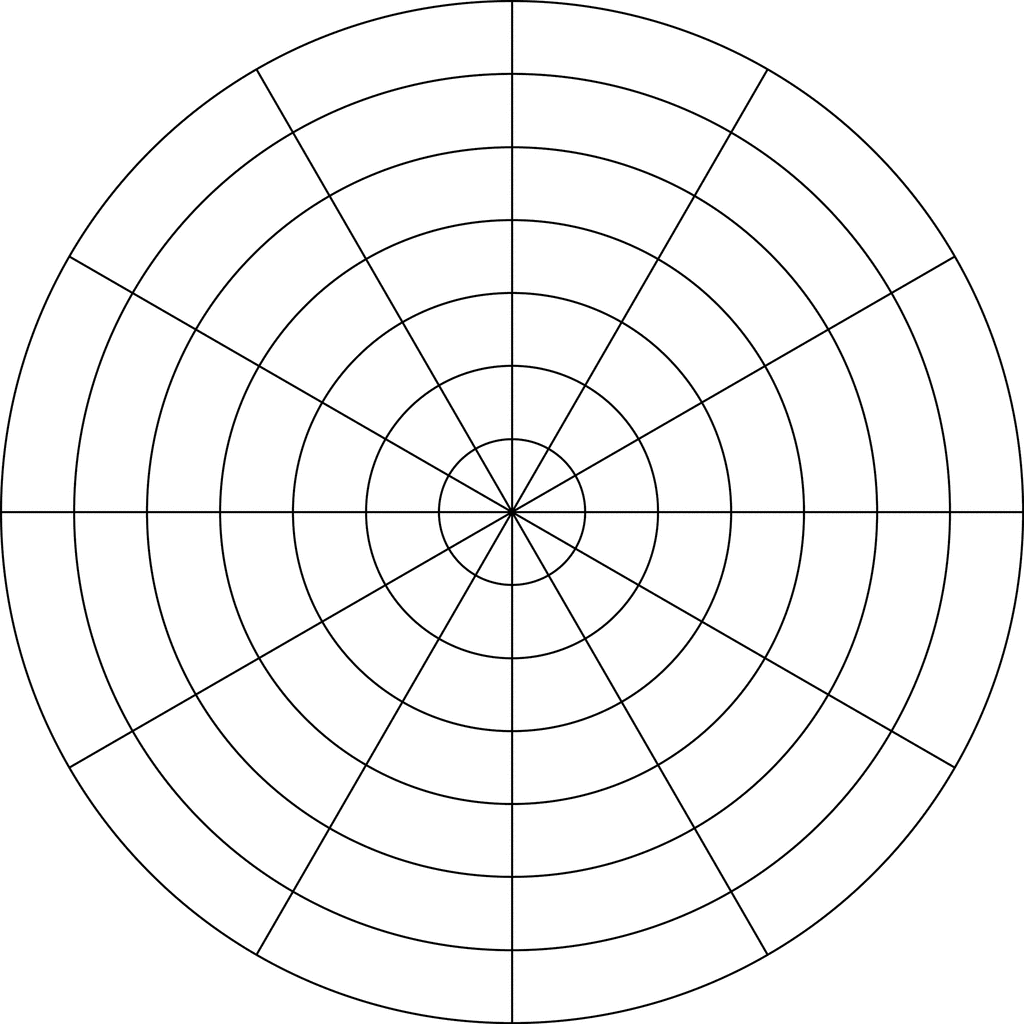
\includegraphics[scale=0.25]{coordinate_plane.png}
\end{center}

\subsection*{Coordinate Conversion}

Let the polar axis coincide with the positive $x$-axis and the pole with the origin.

\vfill

\newpage

\Example Find the Cartesian coordinates of the point with polar coordinates $\left(-4,\dfrac{3\pi}{4}\right)$.

\vfill

\Example Find polar coordinates (with $r>0$) of the point with Cartesian coordinates $\left(-4, 4\sqrt{3}\right)$. Also find polar coordinates with $r>0$ for this point.

\vfill

\subsection*{Polar Curves}

The \textbf{graph of a polar equation} $r=f(\theta)$ consists of all points $P$ that have at least one polar representation $(r,\theta)$ whose coordinates satisfy the equation.

\vspace{4mm}

\textbf{Basic Curves}

\vspace{4mm}

$r=a$, Example: $r=3$ \hspace{50mm} $\theta=b$, Example: $\theta=5\pi/6$

\vfill

\newpage

\Example Convert the following equation to Cartesian coordinates. Describe the resulting curve. 

$$r=6\cos\theta+8\sin\theta$$

\vfill

\newpage

\subsection*{Symmetry in Polar Equations}
\begin{itemize}
	\item We have symmetry about the \textbf{\textit{x}-axis (polar axis)} if $(r,\theta)$ is on the graph whenever $(r,-\theta)$ is.
	\item We have symmetry about the \textbf{\textit{y}-axis ($\theta=\pi/2$)} if $(r,\theta)$ is on the graph whenever $(r,\pi-\theta)=(-r,-\theta)$ is.
	\item We have symmetry about \textbf{the origin (the pole)} if $(r,\theta)$ is on the graph whenever $(-r,\theta)=(r,\theta+\pi)$ is. 
\end{itemize}

\vspace{35mm}

\subsection*{Sketching Polar Curves}

\Example Sketch the graph of the polar curve $r=4+4\cos\theta$ using a table of values and symmetry.

\end{document}